\documentclass{standalone}
\usepackage{tikz}
\usetikzlibrary{patterns, positioning}
\usetikzlibrary{shapes.misc}
\usepackage[outline]{contour}
\contourlength{1.5pt} 


\begin{document}
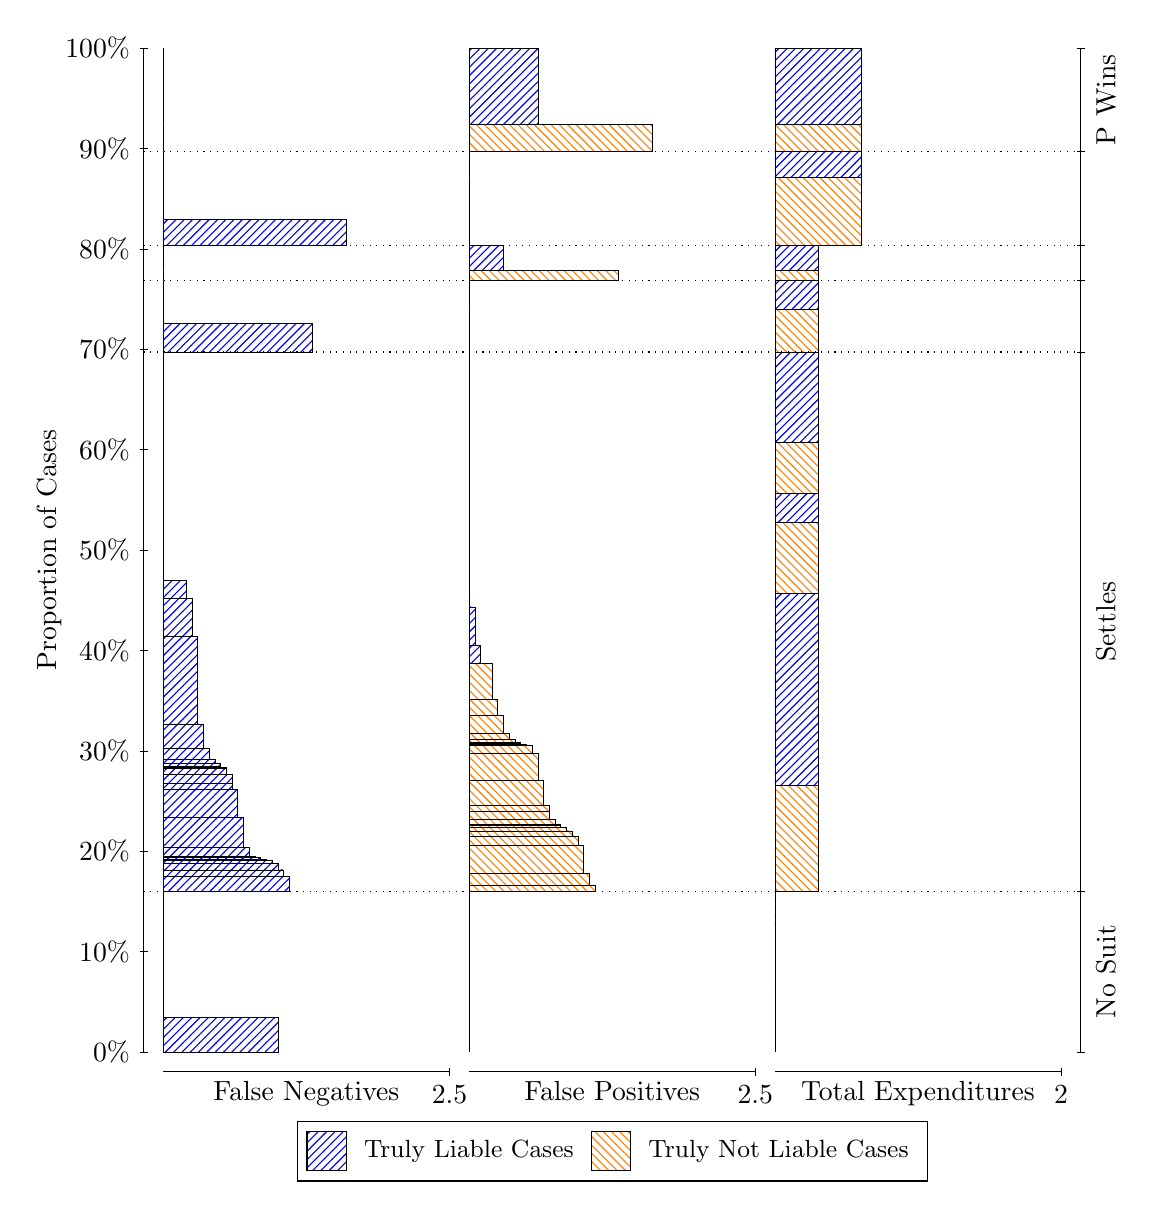
\begin{tikzpicture}
\draw[black, very thin] (1.5,1.75) -- (1.5,14.5);
\node[rotate=90, text=black, anchor=center] at (0.3, 8.125) {Proportion of Cases};
\draw[black, very thin] (1.45,1.75) -- (1.55,1.75);
\node[text=black, anchor=east] at (1.45, 1.75) {0\%};
\draw[black, very thin] (1.45,3.025) -- (1.55,3.025);
\node[text=black, anchor=east] at (1.45, 3.025) {10\%};
\draw[black, very thin] (1.45,4.3) -- (1.55,4.3);
\node[text=black, anchor=east] at (1.45, 4.3) {20\%};
\draw[black, very thin] (1.45,5.575) -- (1.55,5.575);
\node[text=black, anchor=east] at (1.45, 5.575) {30\%};
\draw[black, very thin] (1.45,6.85) -- (1.55,6.85);
\node[text=black, anchor=east] at (1.45, 6.85) {40\%};
\draw[black, very thin] (1.45,8.125) -- (1.55,8.125);
\node[text=black, anchor=east] at (1.45, 8.125) {50\%};
\draw[black, very thin] (1.45,9.4) -- (1.55,9.4);
\node[text=black, anchor=east] at (1.45, 9.4) {60\%};
\draw[black, very thin] (1.45,10.675) -- (1.55,10.675);
\node[text=black, anchor=east] at (1.45, 10.675) {70\%};
\draw[black, very thin] (1.45,11.95) -- (1.55,11.95);
\node[text=black, anchor=east] at (1.45, 11.95) {80\%};
\draw[black, very thin] (1.45,13.225) -- (1.55,13.225);
\node[text=black, anchor=east] at (1.45, 13.225) {90\%};
\draw[black, very thin] (1.45,14.5) -- (1.55,14.5);
\node[text=black, anchor=east] at (1.45, 14.5) {100\%};

\draw[black, very thin] (13.4,1.75) -- (13.4,14.5);
\draw[black, very thin] (13.35,1.75) -- (13.45,1.75);
\node[anchor=west] at (13.35, 1.75) {};
\draw[black, very thin] (13.35,3.7889) -- (13.45,3.7889);
\node[anchor=west] at (13.35, 3.7889) {};
\draw[black, very thin] (13.35,10.639) -- (13.45,10.639);
\node[anchor=west] at (13.35, 10.639) {};
\draw[black, very thin] (13.35,11.546) -- (13.45,11.546);
\node[anchor=west] at (13.35, 11.546) {};
\draw[black, very thin] (13.35,11.99) -- (13.45,11.99);
\node[anchor=west] at (13.35, 11.99) {};
\draw[black, very thin] (13.35,13.187) -- (13.45,13.187);
\node[anchor=west] at (13.35, 13.187) {};
\draw[black, very thin] (13.35,14.5) -- (13.45,14.5);
\node[anchor=west] at (13.35, 14.5) {};

\draw[black, very thin, pattern color=blue, pattern=north east lines] (1.75,1.75) rectangle (3.2033,2.1872);
\draw[black, very thin, pattern color=orange, pattern=north west lines] (1.75,2.1872) rectangle (1.75,3.7889);
\draw[black, very thin, pattern color=blue, pattern=north east lines] (1.75,3.7889) rectangle (3.3487,3.9782);
\draw[black, very thin, pattern color=blue, pattern=north east lines] (1.75,3.9782) rectangle (3.276,4.0633);
\draw[black, very thin, pattern color=blue, pattern=north east lines] (1.75,4.0633) rectangle (3.2033,4.1487);
\draw[black, very thin, pattern color=blue, pattern=north east lines] (1.75,4.1487) rectangle (3.1307,4.1784);
\draw[black, very thin, pattern color=blue, pattern=north east lines] (1.75,4.1784) rectangle (3.058,4.2036);
\draw[black, very thin, pattern color=blue, pattern=north east lines] (1.75,4.2036) rectangle (2.9853,4.2198);
\draw[black, very thin, pattern color=blue, pattern=north east lines] (1.75,4.2198) rectangle (2.9127,4.2235);
\draw[black, very thin, pattern color=blue, pattern=north east lines] (1.75,4.2235) rectangle (2.9127,4.2371);
\draw[black, very thin, pattern color=blue, pattern=north east lines] (1.75,4.2371) rectangle (2.84,4.3451);
\draw[black, very thin, pattern color=blue, pattern=north east lines] (1.75,4.3451) rectangle (2.7673,4.7294);
\draw[black, very thin, pattern color=blue, pattern=north east lines] (1.75,4.7294) rectangle (2.6947,5.0837);
\draw[black, very thin, pattern color=blue, pattern=north east lines] (1.75,5.0837) rectangle (2.622,5.1626);
\draw[black, very thin, pattern color=blue, pattern=north east lines] (1.75,5.1626) rectangle (2.622,5.273);
\draw[black, very thin, pattern color=blue, pattern=north east lines] (1.75,5.273) rectangle (2.5493,5.3591);
\draw[black, very thin, pattern color=blue, pattern=north east lines] (1.75,5.3591) rectangle (2.5493,5.36);
\draw[black, very thin, pattern color=blue, pattern=north east lines] (1.75,5.36) rectangle (2.4767,5.3743);
\draw[black, very thin, pattern color=blue, pattern=north east lines] (1.75,5.3743) rectangle (2.4767,5.4145);
\draw[black, very thin, pattern color=blue, pattern=north east lines] (1.75,5.4145) rectangle (2.404,5.4685);
\draw[black, very thin, pattern color=blue, pattern=north east lines] (1.75,5.4685) rectangle (2.3313,5.6049);
\draw[black, very thin, pattern color=blue, pattern=north east lines] (1.75,5.6049) rectangle (2.2587,5.9073);
\draw[black, very thin, pattern color=blue, pattern=north east lines] (1.75,5.9073) rectangle (2.186,7.0257);
\draw[black, very thin, pattern color=blue, pattern=north east lines] (1.75,7.0257) rectangle (2.1133,7.5126);
\draw[black, very thin, pattern color=blue, pattern=north east lines] (1.75,7.5126) rectangle (2.0407,7.7401);
\draw[black, very thin, pattern color=orange, pattern=north west lines] (1.75,7.7401) rectangle (1.75,10.639);
\draw[black, very thin, pattern color=blue, pattern=north east lines] (1.75,10.639) rectangle (3.6393,11.006);
\draw[black, very thin, pattern color=orange, pattern=north west lines] (1.75,11.006) rectangle (1.75,11.546);
\draw[black, very thin, pattern color=orange, pattern=north west lines] (1.75,11.546) rectangle (1.75,11.674);
\draw[black, very thin, pattern color=blue, pattern=north east lines] (1.75,11.674) rectangle (1.75,11.99);
\draw[black, very thin, pattern color=blue, pattern=north east lines] (1.75,11.99) rectangle (4.0753,12.322);
\draw[black, very thin, pattern color=orange, pattern=north west lines] (1.75,12.322) rectangle (1.75,13.187);
\draw[black, very thin, pattern color=orange, pattern=north west lines] (1.75,13.187) rectangle (1.75,13.529);
\draw[black, very thin, pattern color=blue, pattern=north east lines] (1.75,13.529) rectangle (1.75,14.5);
\draw[black, very thin, pattern color=orange, pattern=north west lines] (5.6333,1.75) rectangle (5.6333,3.3517);
\draw[black, very thin, pattern color=blue, pattern=north east lines] (5.6333,3.3517) rectangle (5.6333,3.7889);
\draw[black, very thin, pattern color=orange, pattern=north west lines] (5.6333,3.7889) rectangle (7.232,3.865);
\draw[black, very thin, pattern color=orange, pattern=north west lines] (5.6333,3.865) rectangle (7.1593,4.0143);
\draw[black, very thin, pattern color=orange, pattern=north west lines] (5.6333,4.0143) rectangle (7.0867,4.3783);
\draw[black, very thin, pattern color=orange, pattern=north west lines] (5.6333,4.3783) rectangle (7.014,4.4936);
\draw[black, very thin, pattern color=orange, pattern=north west lines] (5.6333,4.4936) rectangle (6.9413,4.5582);
\draw[black, very thin, pattern color=orange, pattern=north west lines] (5.6333,4.5582) rectangle (6.8687,4.5975);
\draw[black, very thin, pattern color=orange, pattern=north west lines] (5.6333,4.5975) rectangle (6.796,4.6271);
\draw[black, very thin, pattern color=orange, pattern=north west lines] (5.6333,4.6271) rectangle (6.796,4.6374);
\draw[black, very thin, pattern color=orange, pattern=north west lines] (5.6333,4.6374) rectangle (6.7233,4.6382);
\draw[black, very thin, pattern color=orange, pattern=north west lines] (5.6333,4.6382) rectangle (6.7233,4.7086);
\draw[black, very thin, pattern color=orange, pattern=north west lines] (5.6333,4.7086) rectangle (6.6507,4.806);
\draw[black, very thin, pattern color=orange, pattern=north west lines] (5.6333,4.806) rectangle (6.6507,4.8802);
\draw[black, very thin, pattern color=orange, pattern=north west lines] (5.6333,4.8802) rectangle (6.578,5.2026);
\draw[black, very thin, pattern color=orange, pattern=north west lines] (5.6333,5.2026) rectangle (6.5053,5.5454);
\draw[black, very thin, pattern color=orange, pattern=north west lines] (5.6333,5.5454) rectangle (6.4327,5.6426);
\draw[black, very thin, pattern color=orange, pattern=north west lines] (5.6333,5.6426) rectangle (6.36,5.6607);
\draw[black, very thin, pattern color=orange, pattern=north west lines] (5.6333,5.6607) rectangle (6.2873,5.6695);
\draw[black, very thin, pattern color=orange, pattern=north west lines] (5.6333,5.6695) rectangle (6.2873,5.6778);
\draw[black, very thin, pattern color=orange, pattern=north west lines] (5.6333,5.6778) rectangle (6.2147,5.7259);
\draw[black, very thin, pattern color=orange, pattern=north west lines] (5.6333,5.7259) rectangle (6.142,5.797);
\draw[black, very thin, pattern color=orange, pattern=north west lines] (5.6333,5.797) rectangle (6.0693,6.026);
\draw[black, very thin, pattern color=orange, pattern=north west lines] (5.6333,6.026) rectangle (5.9967,6.225);
\draw[black, very thin, pattern color=orange, pattern=north west lines] (5.6333,6.225) rectangle (5.924,6.6874);
\draw[black, very thin, pattern color=blue, pattern=north east lines] (5.6333,6.6874) rectangle (5.7787,6.9148);
\draw[black, very thin, pattern color=blue, pattern=north east lines] (5.6333,6.9148) rectangle (5.706,7.4017);
\draw[black, very thin, pattern color=blue, pattern=north east lines] (5.6333,7.4017) rectangle (5.6333,10.639);
\draw[black, very thin, pattern color=orange, pattern=north west lines] (5.6333,10.639) rectangle (5.6333,11.178);
\draw[black, very thin, pattern color=blue, pattern=north east lines] (5.6333,11.178) rectangle (5.6333,11.546);
\draw[black, very thin, pattern color=orange, pattern=north west lines] (5.6333,11.546) rectangle (7.5227,11.674);
\draw[black, very thin, pattern color=blue, pattern=north east lines] (5.6333,11.674) rectangle (6.0693,11.99);
\draw[black, very thin, pattern color=orange, pattern=north west lines] (5.6333,11.99) rectangle (5.6333,12.856);
\draw[black, very thin, pattern color=blue, pattern=north east lines] (5.6333,12.856) rectangle (5.6333,13.187);
\draw[black, very thin, pattern color=orange, pattern=north west lines] (5.6333,13.187) rectangle (7.9587,13.529);
\draw[black, very thin, pattern color=blue, pattern=north east lines] (5.6333,13.529) rectangle (6.5053,14.5);
\draw[black, very thin, pattern color=orange, pattern=north west lines] (9.5167,1.75) rectangle (9.5167,3.3517);
\draw[black, very thin, pattern color=blue, pattern=north east lines] (9.5167,3.3517) rectangle (9.5167,3.7889);
\draw[black, very thin, pattern color=orange, pattern=north west lines] (9.5167,3.7889) rectangle (10.062,5.1352);
\draw[black, very thin, pattern color=blue, pattern=north east lines] (9.5167,5.1352) rectangle (10.062,7.5772);
\draw[black, very thin, pattern color=orange, pattern=north west lines] (9.5167,7.5772) rectangle (10.062,8.4764);
\draw[black, very thin, pattern color=blue, pattern=north east lines] (9.5167,8.4764) rectangle (10.062,8.8449);
\draw[black, very thin, pattern color=orange, pattern=north west lines] (9.5167,8.8449) rectangle (10.062,9.4979);
\draw[black, very thin, pattern color=blue, pattern=north east lines] (9.5167,9.4979) rectangle (10.062,10.639);
\draw[black, very thin, pattern color=orange, pattern=north west lines] (9.5167,10.639) rectangle (10.062,11.178);
\draw[black, very thin, pattern color=blue, pattern=north east lines] (9.5167,11.178) rectangle (10.062,11.546);
\draw[black, very thin, pattern color=orange, pattern=north west lines] (9.5167,11.546) rectangle (10.062,11.674);
\draw[black, very thin, pattern color=blue, pattern=north east lines] (9.5167,11.674) rectangle (10.062,11.99);
\draw[black, very thin, pattern color=orange, pattern=north west lines] (9.5167,11.99) rectangle (10.607,12.856);
\draw[black, very thin, pattern color=blue, pattern=north east lines] (9.5167,12.856) rectangle (10.607,13.187);
\draw[black, very thin, pattern color=orange, pattern=north west lines] (9.5167,13.187) rectangle (10.607,13.529);
\draw[black, very thin, pattern color=blue, pattern=north east lines] (9.5167,13.529) rectangle (10.607,14.5);
\draw[black, dotted] (1.5,3.7889) -- (13.4,3.7889);
\draw[black, dotted] (1.5,10.639) -- (13.4,10.639);
\draw[black, dotted] (1.5,11.546) -- (13.4,11.546);
\draw[black, dotted] (1.5,11.99) -- (13.4,11.99);
\draw[black, dotted] (1.5,13.187) -- (13.4,13.187);
\draw[black, very thin] (1.75,1.5) -- (5.3833,1.5);
\node[text=black, anchor=north] at (3.5667, 1.5) {False Negatives};
\draw[black, very thin] (5.3833,1.45) -- (5.3833,1.55);
\node[text=black, anchor=north] at (5.3833, 1.45) {2.5};

\draw[black, very thin] (5.6333,1.5) -- (9.2667,1.5);
\node[text=black, anchor=north] at (7.45, 1.5) {False Positives};
\draw[black, very thin] (9.2667,1.45) -- (9.2667,1.55);
\node[text=black, anchor=north] at (9.2667, 1.45) {2.5};

\draw[black, very thin] (9.5167,1.5) -- (13.15,1.5);
\node[text=black, anchor=north] at (11.333, 1.5) {Total Expenditures};
\draw[black, very thin] (13.15,1.45) -- (13.15,1.55);
\node[text=black, anchor=north] at (13.15, 1.45) {2};

\node[text=black, centered, rotate=90] at (13.72, 2.7695) {\contour{white}{No Suit}};
\node[text=black, centered, rotate=90] at (13.72, 7.2137) {\contour{white}{Settles}};



\node[text=black, centered, rotate=90] at (13.72, 13.843) {\contour{white}{P Wins}};

\draw (7.449999999999999,1.5) node[draw=none] (baseCoordinate) {};
\begin{scope}[align=center]
        \matrix[scale=0.5, draw=black, below=0.5cm of baseCoordinate, nodes={draw}, column sep=0.1cm]{
            \node[rectangle, draw, minimum width=0.5cm, minimum height=0.5cm, pattern color=blue, pattern=north east lines] {}; &
            \node[draw=none, font=\small, text=black] (B) {Truly Liable Cases}; &
            \node[rectangle, draw, minimum width=0.5cm, minimum height=0.5cm, pattern color=orange, pattern=north west lines] {}; &
            \node[draw=none, font=\small, text=black] (B) {Truly Not Liable Cases}; \\
            };
\end{scope}

\end{tikzpicture}
\end{document}